%we need to cite stuff here 
%~\cite{adhocmsgferry}
%~\cite{hybrid}
%~\cite{Routing}
%~\cite{wearable}
%~\cite{QoSrouting}
%~\cite{efficientrouting}
%~\cite{implement}
%~\cite{book1}
%slides -> report
%2 is 1
%1 is 3
%3 is 2

\chapter{Introduction} 

\section{Background}
Message ferrying is a networking approach where data is physically carried between network nodes which cannot communicate directly.
It is sometimes called "store-carry-forward" routing~\cite{Routing}.
Message ferries can be of two types; message oriented ferries and task oriented ferries~\cite{hybrid}.
Message oriented ferries are ferries dedicated to the task of transporting data, known in this context as messages, and their position is controlled by a ferrying algorithm.  
Task oriented ferries transport data but do so while performing another task.
Their movement is not controlled by the ferrying algorithm.
Much past research has focused on message oriented ferries within partitioned, wireless ad-hoc networks~\cite{Routing}~\cite{adhocmsgferry}	.
Very little research has been found on the topic of task oriented ferries, the focus of this project.
Related networking concepts are presented in \ref{sec:net_types}.
Potential examples of applications suitable for message ferrying are presented in section \ref{sec:motivations}.

%The following sections will discuss furthermore about the different type of networks where message ferrying is applicable to.

\subsection{Ad Hoc Network Types}
\label{sec:net_types}

\subsubsection{Mobile Ad Hoc Networks}
A mobile ad hoc network (MANET),  is a self-configuring mesh network of mobile devices connected by wireless links~\cite{book1}.
These mobile devices are free to move independently in any direction and act as a router, where it must forward traffic unrelated to its own.
Much past research on message ferrying has focused on MANETs.

\subsubsection{Partitioned Networks}
\label{sec:clustering}
Partitioned networks are networks with no single hop or multiple hop route between some or even all node pairs.~\cite{hybrid}
In a partitioned network, nodes may remain fully disconnected or they may \emph{cluster}, forming subnetworks in which all nodes are connected.
All current used routing algorithms used in MANETs %TODO: list algorithms?
fail in the presence of partitioning~\cite{Routing}.
This project assumes disconnected nodes, but does not assume nodes cluster.
%TODO: Last sentence is bad

\subsubsection{Delay Tolerant Networks}
\label{sec:delay_loss_tolerant}
%This section is pretty lame
A delay tolerant network is one in which routing strategies and applications must tolerate significant delays delivering packets.
This delay may range from a few minutes up to hours or even days~\cite{Routing}.
%TODO: Current algorithms - bad
The network presented in this report is inherently delay tolerant.

\subsection{Message Ferrying \& Store-Carry-Forward Routing}
\label{sec:ferrying_overview}
Message ferrying is a technique where mobile nodes in a MANET buffer data and physically carry it between nodes which are unable to communicate directly~\cite{adhocmsgferry}.
Store-carry-forward routing is a strategy which makes use of, typically, known or assigned trajectories of these mobile nodes, known as message ferries~\cite{Routing}.
Some messages are dropped if no route to the destination can be found~\cite{implement}.

\section{Motivations and Potential Applications}
\label{sec:motivations}

With the increasing numbers of mobile devices today, such as smartphones, laptops, tablets, netbooks, and more, there are many devices which could be potentially used as message ferries~\cite{wearable}.
This project proposes one way to make use of the significant amount of technology we transport with us on a daily basis.
A message ferrying network could potentially transport small amounts of data over large distances essentially for free~\cite{efficientrouting}.
Beyond the use of message ferrying in remote sensor networks, discussed throughout this report, other applications of this technique might include tracking road traffic conditions, in-house utility management, automation for home devices, industrial monitoring, robot to robot communication and more~\cite{book1}.

%Some of these ideas are good but dont really fit in this section:
%The use of these mesh networks must have low-cost, very low power consumption,low data rate, cheap installation, flexibility, and increase connectivity to make it worthwhile in most cases.

\section{Project Goals}

Message ferrying has typically been examined within the context of improving throughput, reducing delay and increasing reliability within an ad hoc network.
Due to the complexity of incorporating message ferrying into existing ad hoc and MANET routing algorithms, this project will focus on a network in which data is transported strictly using ferries.
No clustering of network nodes and routing within subnetworks will be considered (as presented in section \ref{sec:clustering}).
Surprisingly, very little research has been found for a network with these characteristics.
The goals of this project may be listed as follows.

\begin{itemize}
\item Design and implement a message ferrying algorithm.
\item Simulate this algorithm in a highly partitioned network without node clustering or subnetworks.
\item Evaluate the network using delay and message loss.
\item Examine the impact of node density, ferry count, and limited ferry memory.
\end{itemize}


%An overview look of our architecture:
%
%\begin{figure}[h]
%    \centering
%    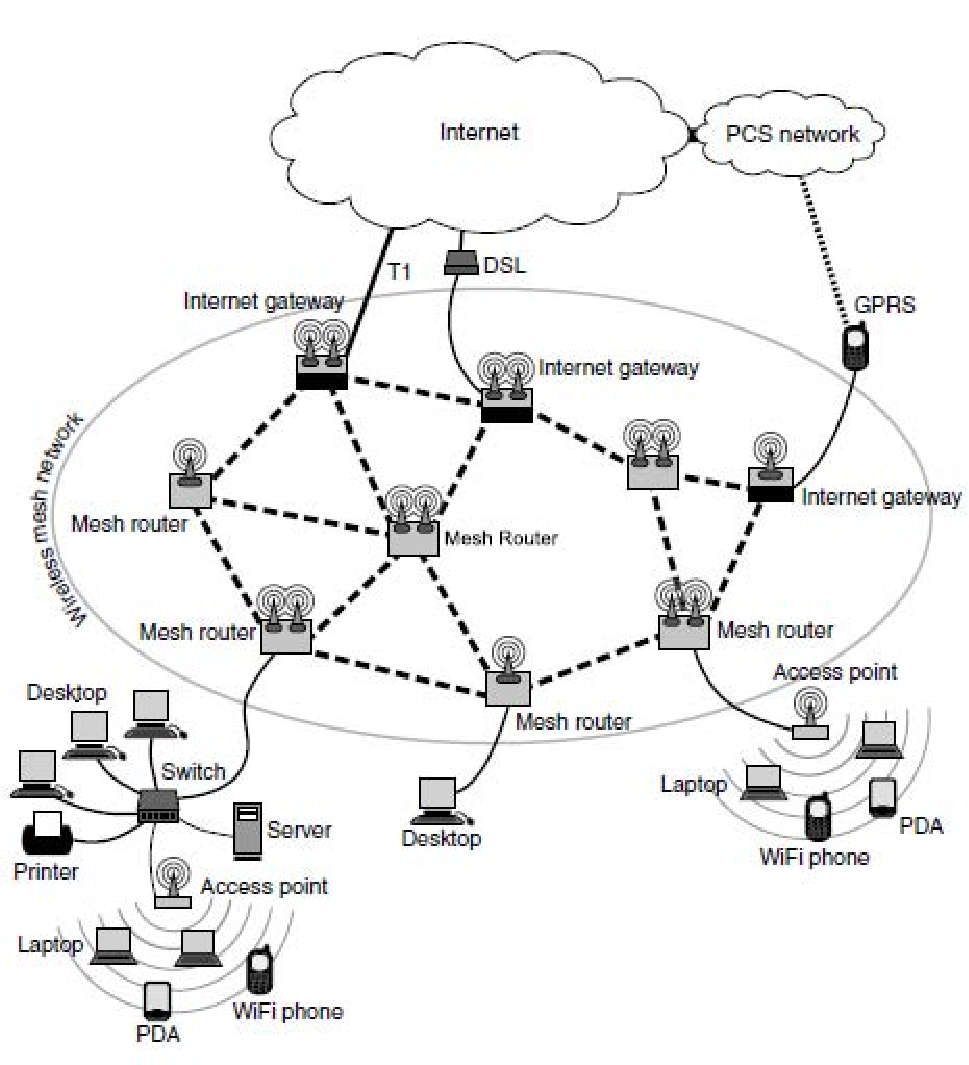
\includegraphics[width=.5\textwidth]{images/wmn_general}
%    \caption{Wireless Mesh Network General Architecture Overview~\cite{book1}}
%    \label{fig:wmn_general}
%\end{figure}
%
%if something referring to this figure, use this \ref{fig:wmn_general}
